\graphicspath{{../images/algorithm/}}
\chapter{Экспериментальные результаты}
\todo{глава не готова}
\section{Пример работы алгоритма}
Для оценки корректности работы алгоритма на каждом из этапов проводился визуальный контроль выбираемых аминокислот с использованием средств визуализации приложения PyMol ~\cite{pymol}.

Я беру непрерывные фрагменты структуры, которые не определяются как $\alpha$-спирали или $\beta$-листы, выбираю среди них те, в которые попадает какая-либо аминокислота, ну и добавляю их к выделяемому контуру - технической сложности никакой.

Далее несколько скриншотов с L и H цепями антитела (2OSL.pdb, но без воды) с разных ракурсов.
\begin{itemize}

\item желтым цветом - L-цепь, на ней голубым выделены аминокислоты, содержащие атомы, которые попали в начальное отобранное множество треугольников выпуклой оболочки

\item Синим - то, что выделилось в результате поиска карманов

\item Красным - фрагменты цепи, которые были добавлены в результате добавления петель

\end{itemize}

Здесь все почти хорошо, но смущает сине-желтый кусок - но это надо поиск карманов смотреть и переделывать. И еще \textbf{сильно смущает} петля прямо по центру - у нее синие края справа и слева, при этом посередине она желтая

\resizebox{0.8\textwidth}{!}{
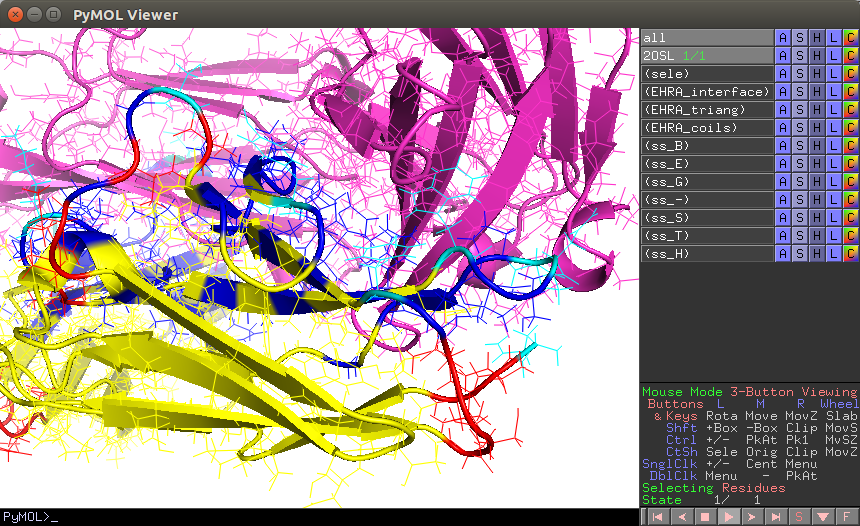
\includegraphics{loops1.png}
}

\resizebox{0.8\textwidth}{!}{
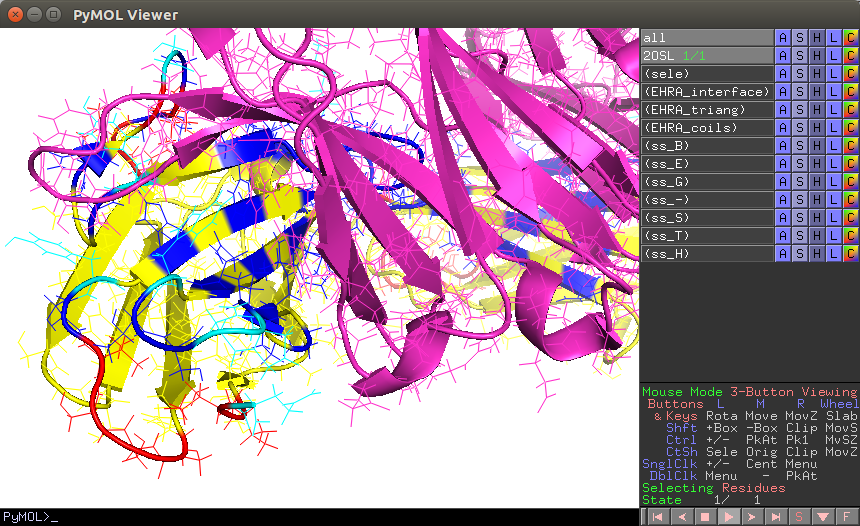
\includegraphics{loops2.png}
}

Здесь снизу явно попала петля, которая удалена от интерфейса взаимодействия, но при этом один из атомов ее аминокислот по удачному стечению обстоятельств попал в множество отобранных треугольников выпуклой оболочки, за счет чего петля попала целиком.

Над этой петлей есть петля, которая вроде бы не влияет вообще. 

\todo{И это наводит на мысль о том, что изначальный выбор аминокислот не так хорош. Возможно, стоит использовать граф Габриэля? }

\resizebox{0.8\textwidth}{!}{
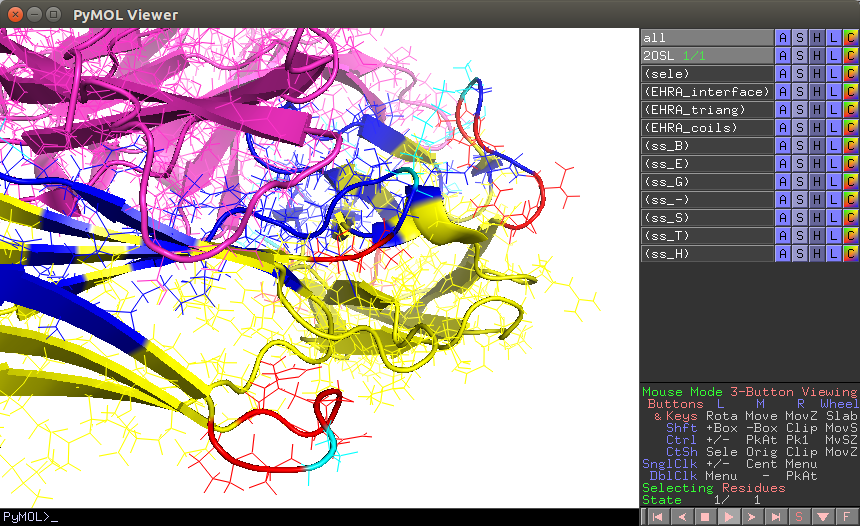
\includegraphics{loops3.png}
}

Посередине петля полностью желтая - но это из-за способа, которым добавлялись карманы.

\resizebox{0.8\textwidth}{!}{
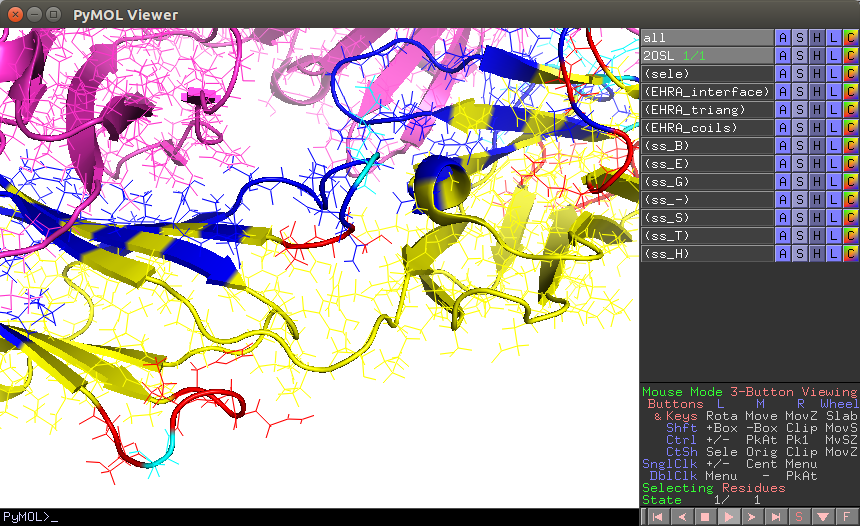
\includegraphics{loops4.png}
}

\newpage
\section{Протокол аланинового сканирования}
% http://www.bakerlab.org/system/files/kortemme04B.pdf
% - картинка отсюда с страницы 3
\todo{-нужна картинка про rosetta alascan protocol }

В работе \cite{kortemme2002} показано, что (сказать про функцию энергии для компьютерного моделирования аланинового сканирования)

\todo{-описание того, в какой части предполагается использовать модиф регионы}
\vspace{10cm}
\section{Сравнение с другими инструментами}
Уже обработанные данные есть здесь: \cite{kortemme_alascan_datasets}

Картинка \cite{benchmark_img} но я не уверена, можно ли ее приводить без разрешения

\todo{- картинка с схемой работы скрипта}

\todo{- красивая табличка, с процентом аминокислот в цепочке, попавших в регион, а также попавшими и не попавшими хотспотами.}
%Описание таблички (нужно для корректного вывода в скрипте)
% 1. идентификатор файла pdb
% 2. мутируемая цепь
% 3. цепь\ лиганд, взаимодействие с которым оценивается
% 4. длина цепочки, длина региона, число замаскированных амк
% 5. 
\\
\todo{-написать скрипт, который для данного pdb и пары цепочек проводит ala-scan по всем позициям и сравнивает методы, которые используются для фильтрации аминокислот.}

\todo{сделать табличку по данным asedb и bid, 

и для того, что нет (хотспоты искать с помощью протокола аланинового сканирования, в табличке рисовать циферки).

если есть амк, которые не нашлись,}
\vspace{10cm}



